\documentclass[14pt]{extbook}
\usepackage{multicol, enumerate, enumitem, hyperref, color, soul, setspace, parskip, fancyhdr} %General Packages
\usepackage{amssymb, amsthm, amsmath, latexsym, units, mathtools} %Math Packages
\everymath{\displaystyle} %All math in Display Style
% Packages with additional options
\usepackage[headsep=0.5cm,headheight=12pt, left=1 in,right= 1 in,top= 1 in,bottom= 1 in]{geometry}
\usepackage[usenames,dvipsnames]{xcolor}
\usepackage{dashrule}  % Package to use the command below to create lines between items
\newcommand{\litem}[1]{\item#1\hspace*{-1cm}\rule{\textwidth}{0.4pt}}
\pagestyle{fancy}
\lhead{Progress Quiz 8}
\chead{}
\rhead{Version C}
\lfoot{5493-4176}
\cfoot{}
\rfoot{Summer C 2021}
\begin{document}

\begin{enumerate}
\litem{
Choose the equation of the function graphed below.
\begin{center}
    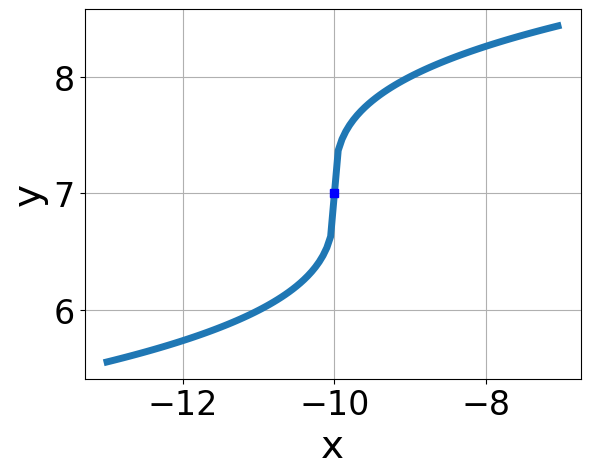
\includegraphics[width=0.5\textwidth]{../Figures/radicalGraphToEquationC.png}
\end{center}
\begin{enumerate}[label=\Alph*.]
\item \( f(x) = - \sqrt[3]{x - 10} + 7 \)
\item \( f(x) = \sqrt[3]{x - 10} + 7 \)
\item \( f(x) = \sqrt[3]{x + 10} + 7 \)
\item \( f(x) = - \sqrt[3]{x + 10} + 7 \)
\item \( \text{None of the above} \)

\end{enumerate} }
\litem{
Solve the radical equation below. Then, choose the interval(s) that the solution(s) belongs to.\[ \sqrt{-20 x^2 - 24} - \sqrt{47 x} = 0 \]\begin{enumerate}[label=\Alph*.]
\item \( x_1 \in [0.24, 2.82] \text{ and } x_2 \in [-0.2,1.5] \)
\item \( \text{All solutions lead to invalid or complex values in the equation.} \)
\item \( x \in [-2.16,-1.15] \)
\item \( x \in [-1.47,0.11] \)
\item \( x_1 \in [-2.16, -1.15] \text{ and } x_2 \in [-2.9,0.3] \)

\end{enumerate} }
\litem{
What is the domain of the function below?\[ f(x) = \sqrt[4]{-7 x - 4} \]\begin{enumerate}[label=\Alph*.]
\item \( (-\infty, a], \text{ where } a \in [-1.5, 4.7] \)
\item \( [a, \infty), \text{where } a \in [-1, 1.3] \)
\item \( (-\infty, \infty) \)
\item \( [a, \infty), \text{where } a \in [-3.9, -1] \)
\item \( (-\infty, a], \text{where } a \in [-1.9, -1.3] \)

\end{enumerate} }
\litem{
Choose the graph of the equation below.\[ f(x) = \sqrt[3]{x - 6} - 7 \]\begin{enumerate}[label=\Alph*.]
\begin{multicols}{2}\item 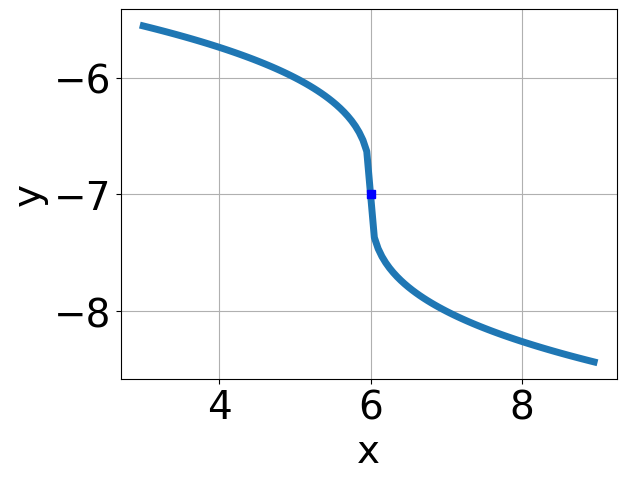
\includegraphics[width = 0.3\textwidth]{../Figures/radicalEquationToGraphCopyAC.png}\item 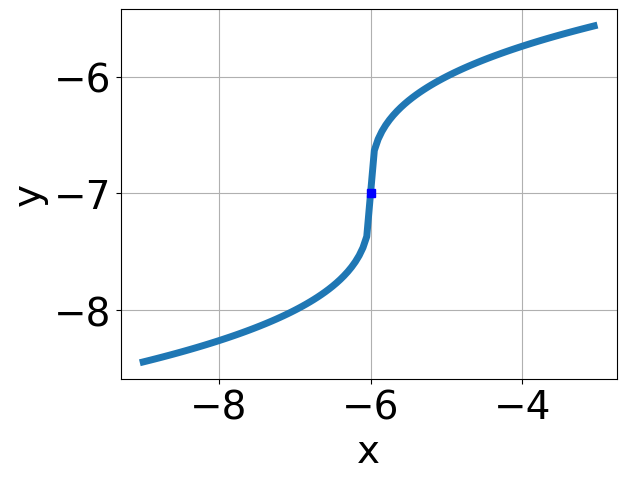
\includegraphics[width = 0.3\textwidth]{../Figures/radicalEquationToGraphCopyBC.png}\item 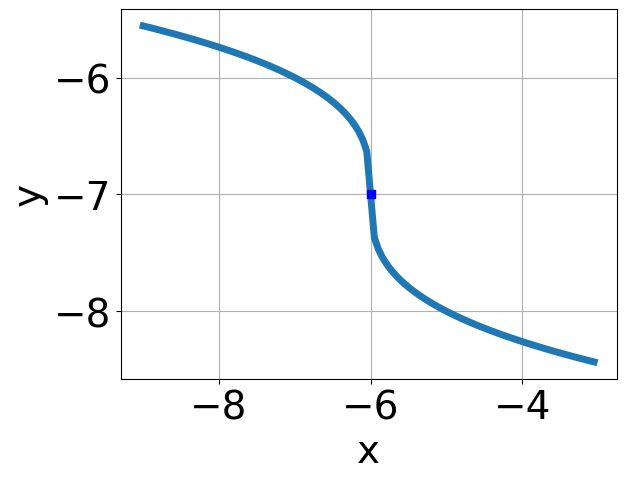
\includegraphics[width = 0.3\textwidth]{../Figures/radicalEquationToGraphCopyCC.png}\item 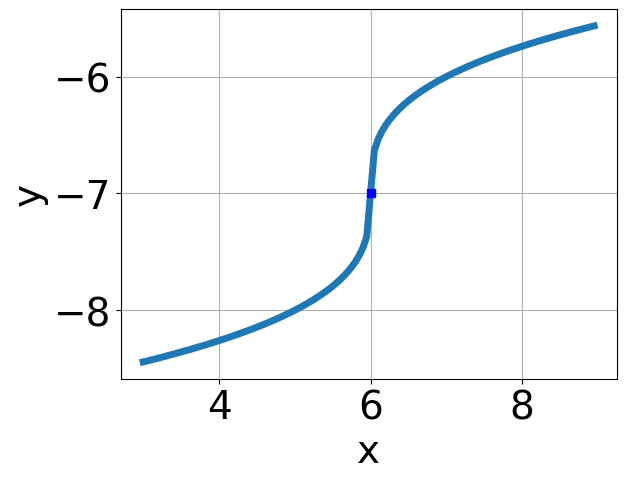
\includegraphics[width = 0.3\textwidth]{../Figures/radicalEquationToGraphCopyDC.png}\end{multicols}\item None of the above.
\end{enumerate} }
\litem{
Solve the radical equation below. Then, choose the interval(s) that the solution(s) belongs to.\[ \sqrt{9 x - 3} - \sqrt{-2 x + 7} = 0 \]\begin{enumerate}[label=\Alph*.]
\item \( x_1 \in [-0.07, 0.35] \text{ and } x_2 \in [3.5,4.5] \)
\item \( x_1 \in [-0.07, 0.35] \text{ and } x_2 \in [-2.09,1.91] \)
\item \( x \in [0.52,1.09] \)
\item \( \text{All solutions lead to invalid or complex values in the equation.} \)
\item \( x \in [-0.5,-0.15] \)

\end{enumerate} }
\litem{
Choose the equation of the function graphed below.
\begin{center}
    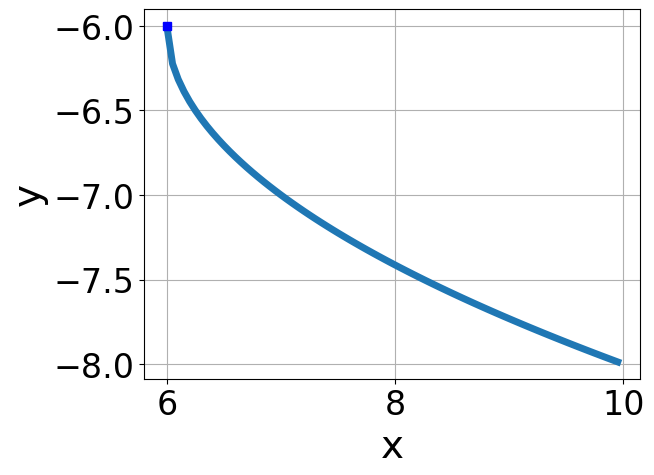
\includegraphics[width=0.5\textwidth]{../Figures/radicalGraphToEquationCopyC.png}
\end{center}
\begin{enumerate}[label=\Alph*.]
\item \( f(x) = \sqrt[3]{x + 6} - 6 \)
\item \( f(x) = \sqrt[3]{x - 6} - 6 \)
\item \( f(x) = - \sqrt[3]{x + 6} - 6 \)
\item \( f(x) = - \sqrt[3]{x - 6} - 6 \)
\item \( \text{None of the above} \)

\end{enumerate} }
\litem{
Solve the radical equation below. Then, choose the interval(s) that the solution(s) belongs to.\[ \sqrt{9 x + 8} - \sqrt{6 x + 6} = 0 \]\begin{enumerate}[label=\Alph*.]
\item \( x_1 \in [-1.1, -1] \text{ and } x_2 \in [-1.46,-0.82] \)
\item \( x \in [-4.88,-4.46] \)
\item \( x_1 \in [-0.89, -0.83] \text{ and } x_2 \in [-0.73,-0.45] \)
\item \( \text{All solutions lead to invalid or complex values in the equation.} \)
\item \( x \in [-0.77,-0.5] \)

\end{enumerate} }
\litem{
What is the domain of the function below?\[ f(x) = \sqrt[4]{-6 x - 9} \]\begin{enumerate}[label=\Alph*.]
\item \( [a, \infty), \text{where } a \in [-0.8, 1.4] \)
\item \( (-\infty, a], \text{ where } a \in [-2.8, -1.14] \)
\item \( [a, \infty), \text{where } a \in [-2.7, -0.7] \)
\item \( (-\infty, a], \text{where } a \in [-1.36, 0.56] \)
\item \( (-\infty, \infty) \)

\end{enumerate} }
\litem{
Choose the graph of the equation below.\[ f(x) = - \sqrt[3]{x + 14} + 3 \]\begin{enumerate}[label=\Alph*.]
\begin{multicols}{2}\item 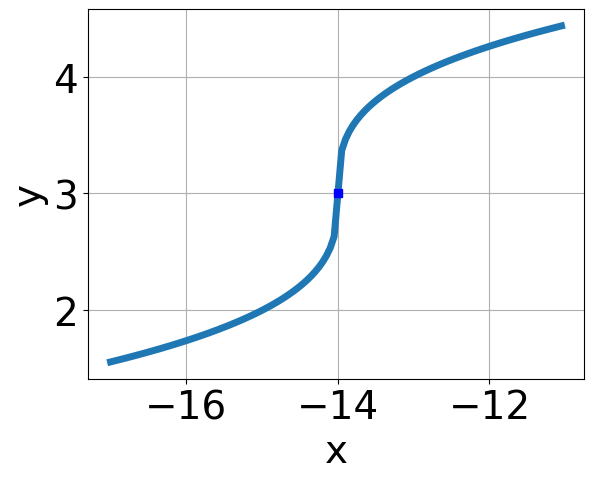
\includegraphics[width = 0.3\textwidth]{../Figures/radicalEquationToGraphAC.png}\item 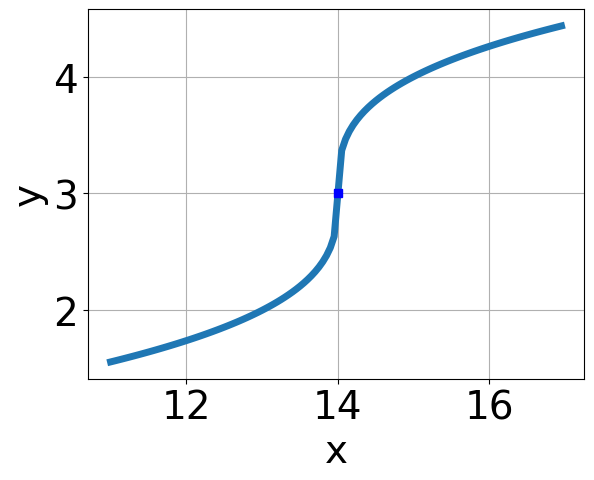
\includegraphics[width = 0.3\textwidth]{../Figures/radicalEquationToGraphBC.png}\item 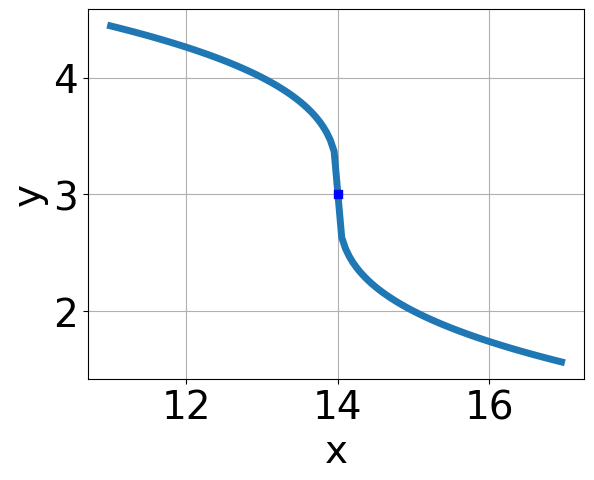
\includegraphics[width = 0.3\textwidth]{../Figures/radicalEquationToGraphCC.png}\item 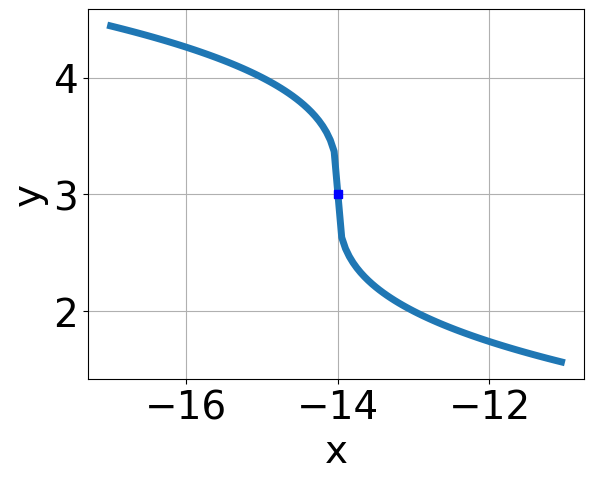
\includegraphics[width = 0.3\textwidth]{../Figures/radicalEquationToGraphDC.png}\end{multicols}\item None of the above.
\end{enumerate} }
\litem{
Solve the radical equation below. Then, choose the interval(s) that the solution(s) belongs to.\[ \sqrt{16 x^2 - 18} - \sqrt{-12 x} = 0 \]\begin{enumerate}[label=\Alph*.]
\item \( x \in [-2.2,-0.4] \)
\item \( \text{All solutions lead to invalid or complex values in the equation.} \)
\item \( x_1 \in [0.5, 1.2] \text{ and } x_2 \in [1.17,1.59] \)
\item \( x \in [0.5,1.2] \)
\item \( x_1 \in [-2.2, -0.4] \text{ and } x_2 \in [-0.12,1.42] \)

\end{enumerate} }
\end{enumerate}

\end{document}